\section{Thiết kế và môi trường thực
nghiệm}\label{sec:thietke}

\subsection{Nguyên mẫu Data
Pipeline}\label{sec:nguyenmau}

Nguyên mẫu triển khai một pipeline phân tích gồm bốn giai đoạn: Source,
Bronze, Silver và Gold. Dữ liệu nguồn được sinh tổng hợp bằng random
seed cố định nhằm hỗ trợ khả năng tái lập. Bronze lưu dữ liệu sau khi
nạp dữ liệu, Silver thực hiện chuẩn hóa và transformation, còn Gold lưu kết
quả tổng hợp phục vụ phân tích. Mỗi giai đoạn sinh ra bằng chứng integrity
và ghi vào ledger.

Đối với mỗi giai đoạn, ledger ghi nhận giai đoạn name, số lượng bản ghi, schema
hash, batch hash, block hash, previous block hash, transformation
siêu dữ liệu, dấu thời gian và định danh lần chạy pipeline. Batch hash đại diện cho
nội dung đã chuẩn hóa chính tắc của output tại giai đoạn. Schema hash đại diện cho
cấu trúc dữ liệu. Block hash là giá trị băm (digest) mật mã của nội dung trong block.
Previous hash liên kết block hiện tại với block trước đó trong cùng
pipeline run.

\begin{figure}[t]
\centering
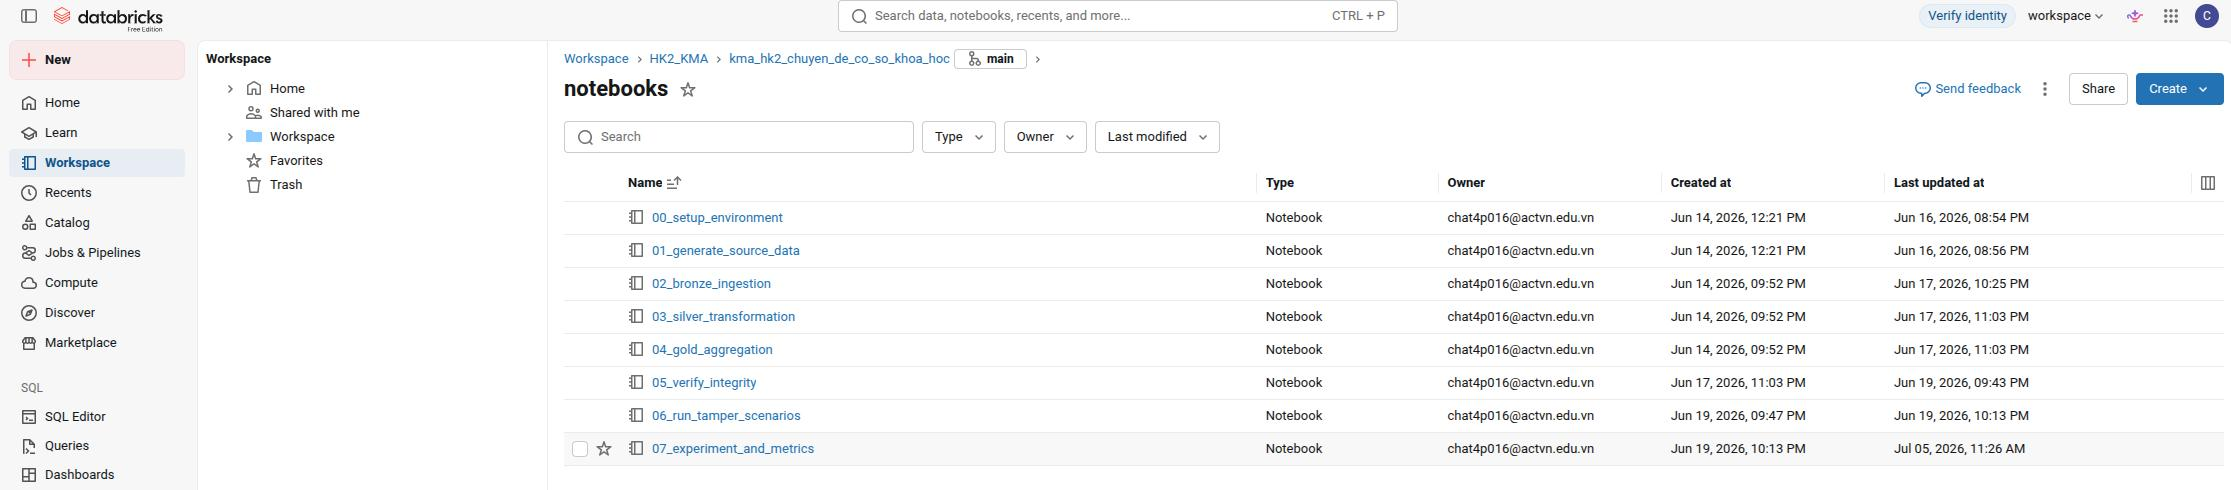
\includegraphics[width=\columnwidth]{images/screenshots/databricks_workspace_real.pdf}
\caption{Môi trường triển khai thực nghiệm trên Databricks Free Edition: các notebook \texttt{00\_setup\_environment} đến \texttt{07\_experiment\_and\_metrics} trong thư mục \texttt{notebooks}, đồng bộ từ repo Git nhánh \texttt{main}, thực thi tuần tự luồng Source--Bronze--Silver--Gold (repo: \url{https://github.com/sonnntech/kma_hk2_chuyen_de_co_so_khoa_hoc}).}
\label{fig:databricks-env}
\end{figure}

Verification engine tính toán lại bằng chứng ở từng giai đoạn và so sánh với
ledger đã lưu. Sai lệch mã băm nội dung chỉ ra khả năng data tampering. Sai
lệch số lượng bản ghi chỉ ra khả năng chèn hoặc xóa. Sai lệch block
nội dung chỉ ra ledger tampering. Sai lệch previous hash chỉ ra chain
link bị phá vỡ.

\subsection{Tamper Scenarios}\label{tamper-scenarios}

Nghiên cứu đánh giá sáu tamper scenarios và một clean scenario. Clean
scenario, ký hiệu NONE, được dùng để quan sát false positive. Các tamper
scenarios bao gồm sửa giá trị giao dịch, xóa bản ghi, chèn bản ghi giả,
sửa batch hash đã lưu, sửa transformation siêu dữ liệu và sửa previous-hash
link. Bảng~\ref{tab:scenarios} liệt kê từng scenario cùng verification
outcome kỳ vọng.

\begin{table}[!t]
\centering
\footnotesize
\caption{Tamper scenarios và outcome kỳ vọng}
\label{tab:scenarios}
\begin{tabular}{|p{3.9cm}|p{3.4cm}|}
\hline
\textbf{Scenario} & \textbf{Outcome kỳ vọng} \\
\hline
NONE & VALID \\
\hline
MODIFY\_\allowbreak TRANSACTION\_\allowbreak AMOUNT & DATA\_\allowbreak TAMPERED \\
\hline
DELETE\_\allowbreak TRANSACTION & RECORD\_\allowbreak COUNT\_\allowbreak MISMATCH \\
\hline
INSERT\_\allowbreak FAKE\_\allowbreak TRANSACTION & RECORD\_\allowbreak COUNT\_\allowbreak MISMATCH \\
\hline
MODIFY\_\allowbreak LEDGER\_\allowbreak BATCH\_\allowbreak HASH & DATA\_\allowbreak TAMPERED \\
\hline
MODIFY\_\allowbreak LEDGER\_\allowbreak TRANSFORMATION & BLOCK\_\allowbreak TAMPERED \\
\hline
MODIFY\_\allowbreak LEDGER\_\allowbreak PREVIOUS\_\allowbreak HASH & CHAIN\_\allowbreak BROKEN \\
\hline
\end{tabular}
\end{table}
\subsection{Quy trình thực
nghiệm}\label{sec:quytrinh}

Quy trình thực nghiệm được mô tả trong
Hình~\ref{fig:procedure}. Đầu tiên, môi trường và các
Delta tables được khởi tạo. Tiếp theo, dữ liệu synthetic được sinh bằng
seed cố định. Sau đó, pipeline baseline và pipeline có treatment được
thực thi. Verification engine kiểm tra clean run. Một tamper scenario
được áp dụng, rồi verification được chạy lại để đo detection và
traceability. Trạng thái baseline được reset trước khi chuyển sang
scenario tiếp theo. Cuối cùng, benchmark được chạy theo nhiều mức record
count.

\begin{figure}[t]
\centering
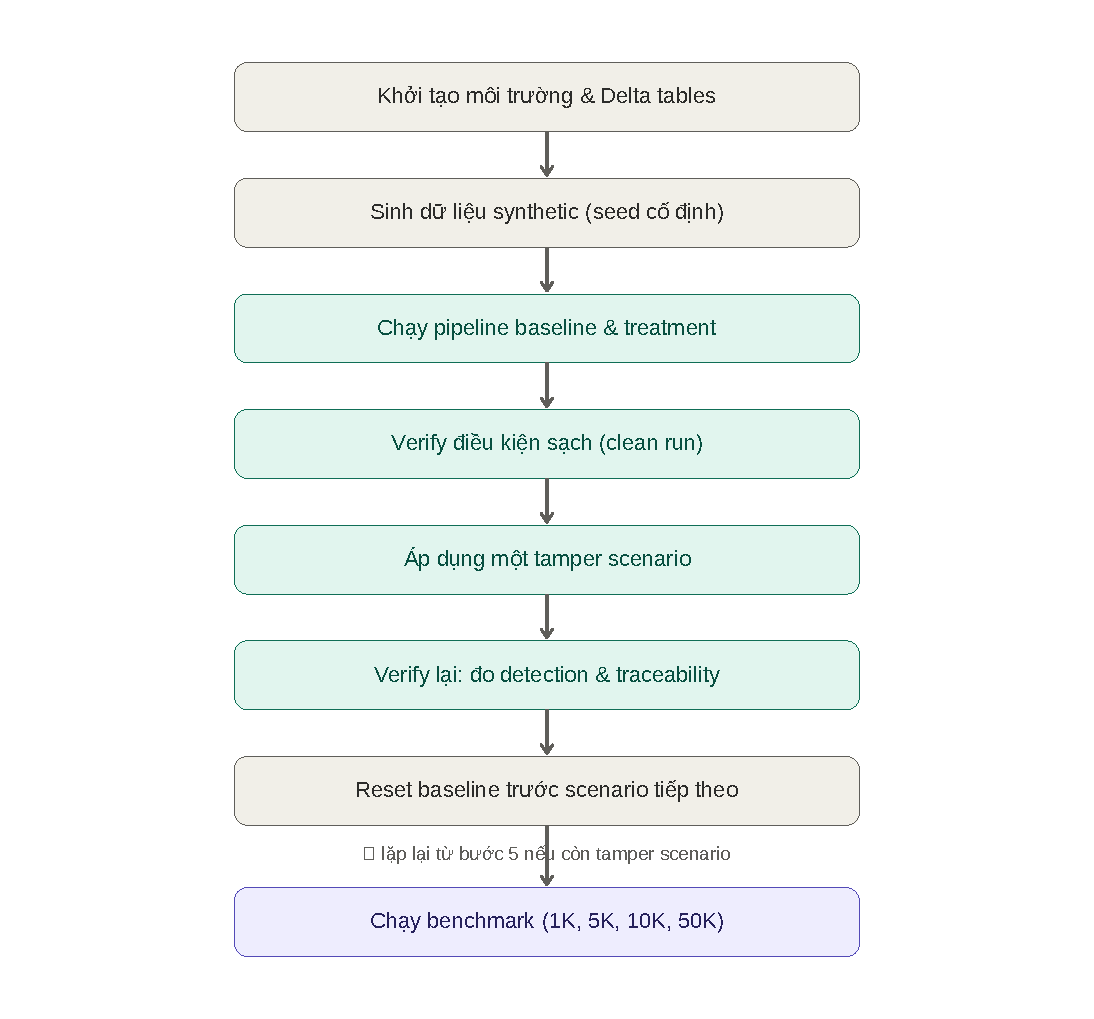
\includegraphics[width=\columnwidth]{images/quy_trinh_thuc_nghiem.pdf}
\caption{Quy trình thực nghiệm cho clean run, tamper run và benchmark run.}
\label{fig:procedure}
\end{figure}

Các lần chạy khởi động (warm-up) được đánh dấu và loại khỏi phần tổng hợp benchmark
chính. Median chi phí phát sinh được ưu tiên hơn mean vì trạng thái cloud compute
và khởi động nguội (cold start) có thể tạo giá trị ngoại lai. Benchmark sử dụng các mức số lượng bản ghi
1K, 5K, 10K và 50K.

\FloatBarrier
